% !TEX program = lualatex
%% FullCourse_10Lecs -- Lecture 2, Topic 2.2:
%% Language, Generation, and Agency
%% NOTE: build this deck with lualatex (it renders the Chinese terms via luatexja+Fandol);
%% under pdflatex it still compiles, substituting pinyin for the CJK glyphs.
%% Generative-stack deck of the Lec02 split. Reuses the intelligence/NLP/LLM/
%% how-people-use frames from the old Lec02_T1_Evolution_Pillars.tex, plus the
%% taxonomy-recap and Lec3 lead-in from the old Lec02_T2; adds the AI Snake Oil
%% generative-failure cautions (Narayanan & Kapoor, 2024).

%% Shared preamble for the FullCourse_10Lecs topic decks.
%%
%% Each topic .tex \input's this file, then defines its own \title, \date
%% override (if any), \graphicspath, and \begin{document}.
%%
%% Reconstructed verbatim from the inlined copy preserved in
%% Lec10_Case_Studies/Lec10_T8_Case6_DeepRamsey.tex (lines 23-190), which is
%% explicitly annotated there as "from ../shared_preamble.tex, copied verbatim".
%% Base preamble matches MiniCourse_8hr/Slides/shared_preamble.tex; this version
%% additionally provides \sectiondivider, the conceptbox/cautionbox/examplebox/
%% takeawaybox tcolorboxes, and \compacttables used across the split decks.

\documentclass[10pt,english,aspectratio=169]{beamer}

\usepackage{ae,aecompl}
\usepackage[T1]{fontenc}
\usepackage{textcomp}
\usepackage[utf8]{inputenc}
\usepackage{babel}
\usepackage{datetime2}

\setcounter{secnumdepth}{3}
\setcounter{tocdepth}{3}

\usepackage{amsmath, amssymb, amsthm, graphicx}
\usepackage{booktabs, multirow}
\usepackage{tikz}
\usepackage{pgfplots}
\pgfplotsset{compat=1.16}
\usepackage[most]{tcolorbox}
\tcbuselibrary{skins, breakable, theorems}
\usepackage{listings}
\usepackage{xcolor}

\lstset{
  basicstyle=\ttfamily\small,
  keywordstyle=\color{blue!80!black}\bfseries,
  commentstyle=\color{green!50!black}\itshape,
  stringstyle=\color{orange!80!black},
  backgroundcolor=\color{gray!8},
  frame=single,
  rulecolor=\color{gray!40},
  breaklines=true,
  showstringspaces=false,
  numbers=none,
}

\lstdefinestyle{pythonstyle}{
    language=Python,
    basicstyle=\ttfamily\footnotesize,
    keywordstyle=\color{blue!80!black}\bfseries,
    commentstyle=\color{green!50!black}\itshape,
    stringstyle=\color{orange!80!black},
    frame=single,
    breaklines=true,
    showstringspaces=false,
    numbers=left,
    numbersep=5pt,
    numberstyle=\tiny\color{gray},
    backgroundcolor=\color{gray!8},
    rulecolor=\color{gray!40}
}

\ifx\hypersetup\undefined
  \AtBeginDocument{%
    \hypersetup{bookmarks=false,breaklinks=true,pdfborder={0 0 0},colorlinks=true,
      linkcolor=DarkText,urlcolor=RedTitle}%
  }
\else
  \hypersetup{bookmarks=false,breaklinks=true,pdfborder={0 0 0},colorlinks=true,
    linkcolor=DarkText,urlcolor=RedTitle}%
\fi

\makeatletter
\newcommand\makebeamertitle{%
  \begin{frame}[plain]
    \vspace*{1.0cm}
    \centering
    {\usebeamerfont{title}\usebeamercolor[fg]{title}\inserttitle\par}
    \vspace{1.0cm}
    {\usebeamerfont{author}\usebeamercolor[fg]{author}\insertauthor\par}
    \vspace{0.2cm}
    {\usebeamerfont{date}\usebeamercolor[fg]{date}\insertdate\par}
  \end{frame}}%
\AtBeginDocument{%
  \let\origtableofcontents=\tableofcontents
  \def\tableofcontents{\@ifnextchar[{\origtableofcontents}{\gobbletableofcontents}}
  \def\gobbletableofcontents#1{\origtableofcontents}%
}

\usetheme{metropolis}
\usefonttheme{professionalfonts}

\definecolor{LightGray}{RGB}{230,230,230}
\definecolor{RedTitle}{RGB}{0,0,200}
\definecolor{VeryLightGray}{RGB}{245,245,245}
\definecolor{DarkText}{RGB}{0,0,0}

\setbeamercolor{background canvas}{bg=white}
\setbeamercolor{title}{fg=RedTitle}
\setbeamercolor{author}{fg=DarkText}
\setbeamercolor{date}{fg=DarkText}
\setbeamercolor{frametitle}{bg=VeryLightGray,fg=DarkText}
\setbeamercolor{normal text}{fg=DarkText}
\setbeamerfont{title}{size=\large}

\setbeamersize{text margin left=5mm, text margin right=5mm}
\addtobeamertemplate{frametitle}{}{\vspace{-0.5em}}
\newcommand{\reducevspace}{\vspace{-0.5cm}}

% Shared section divider and box styles for split topic decks.
\newcommand{\sectiondivider}[2]{%
\begin{frame}[plain,noframenumbering]
\begin{center}
\vfill
{\Large\textbf{#1}\par}
\vspace{0.35cm}
{\normalsize #2\par}
\vfill
\end{center}
\end{frame}
}

\newtcolorbox{conceptbox}[1][]{
  colback=blue!3,
  colframe=RedTitle!55,
  boxrule=0.35mm,
  arc=1mm,
  left=2mm,
  right=2mm,
  top=1mm,
  bottom=1mm,
  #1
}
\newtcolorbox{cautionbox}[1][]{
  colback=red!3,
  colframe=red!50!black,
  boxrule=0.35mm,
  arc=1mm,
  left=2mm,
  right=2mm,
  top=1mm,
  bottom=1mm,
  #1
}
\newtcolorbox{examplebox}[1][]{
  colback=green!3,
  colframe=green!45!black,
  boxrule=0.35mm,
  arc=1mm,
  left=2mm,
  right=2mm,
  top=1mm,
  bottom=1mm,
  #1
}
\newtcolorbox{takeawaybox}[1][]{
  colback=VeryLightGray,
  colframe=RedTitle!55,
  boxrule=0.35mm,
  arc=1mm,
  left=2mm,
  right=2mm,
  top=1mm,
  bottom=1mm,
  #1
}
\newcommand{\compacttables}{\renewcommand{\arraystretch}{1.15}}

\setbeamertemplate{navigation symbols}{}
\setbeamertemplate{footline}{%
  \hfill%
  \usebeamercolor[fg]{page number in head/foot}%
  \usebeamerfont{page number in head/foot}%
  \insertframenumber\,/\,\inserttotalframenumber\kern1em\vskip2pt%
}

\makeatother

\author{Zhigang Feng}
% "date with time": compile timestamp so each build is identifiable.
\date{\today\ \DTMcurrenttime}


% --- CJK: real characters under Lua/XeLaTeX; pinyin fallback under pdfLaTeX.
%     Force Latin Modern for the Latin text so this deck matches the pdflatex
%     decks (which render Computer Modern); only the CJK glyphs use Fandol. ---
\usepackage{iftex}
\ifluatex
  \usepackage{luatexja-fontspec}
  \setmainfont{Latin Modern Roman}%
  \setsansfont{Latin Modern Sans}%
  \setmonofont{Latin Modern Mono}%
  \setmainjfont{FandolSong-Regular.otf}[BoldFont=FandolHei-Regular.otf]%
  \newcommand{\zhterm}[2]{#1}% lualatex (target engine): real Chinese characters
\else\ifxetex
  \usepackage{fontspec}
  \setmainfont{Latin Modern Roman}%
  \setsansfont{Latin Modern Sans}%
  \setmonofont{Latin Modern Mono}%
  \usepackage{xeCJK}
  \setCJKmainfont{FandolSong-Regular.otf}[BoldFont=FandolHei-Regular.otf]%
  \newcommand{\zhterm}[2]{#1}% xelatex: real Chinese characters
\else
  \newcommand{\zhterm}[2]{#2}% pdflatex (batch build): romanization keeps it compiling
\fi\fi

\graphicspath{{./figures/}{./pic/}{../../MiniCourse_8hr/Slides/Module1_ML_Foundations/pic/}{../}}

% Suppress the redundant auto-generated metropolis section page; the
% \sectiondivider frames below are the dividers we keep.
\metroset{sectionpage=none}
\usetikzlibrary{positioning,arrows.meta,shapes,calc}
%% Lec02 shared MAP slide: "one map, two acts" recurring diagram.
%% Input this file AFTER ../shared_preamble.tex (needs RedTitle, VeryLightGray,
%% DarkText) and AFTER \usetikzlibrary{positioning,arrows.meta,shapes,calc}.
%% Call \LecTwoMap{k} inside a frame, where k in {1,2} highlights the current
%% act ("you are here") and k = 0 renders the closing reprise with both acts
%% checked green (used by T2's closing frame).
%% Filename deliberately does NOT match the build glob Lec*_T*.tex, so the build
%% script never tries to compile it standalone.
%%
%% The two acts are the lecture's story: PREDICT -> GENERATE, i.e. the
%% predictive stack (ML pillars + deep learning + where it fails) and the
%% generative/agentic stack (LLMs + agents + where it fails) --- and the two
%% acts point at the course's two arcs (dynamics: Lec03-06; language: Lec07-09).

\newcommand{\LecTwoMap}[1]{%
% Precompute per-box style selectors; TikZ option lists are comma-split before
% TeX conditionals run, so \ifnum must not sit inside a [...] options list.
\ifnum#1=0
  \tikzset{lmapa/.style={lmapdone}, lmapb/.style={lmapdone}}%
\else
  \tikzset{lmapa/.style={}, lmapb/.style={}}%
  \ifnum#1=1 \tikzset{lmapa/.style={lmapcur}}\fi
  \ifnum#1=2 \tikzset{lmapb/.style={lmapcur}}\fi
\fi
\begin{center}
\begin{tikzpicture}[
    act/.style={rectangle, rounded corners, draw=black!60, fill=VeryLightGray,
        minimum width=4.6cm, minimum height=1.0cm, text width=4.45cm,
        align=center, font=\small, text=DarkText},
    lmapcur/.style={draw=RedTitle, very thick, fill=orange!20},
    lmapdone/.style={draw=green!45!black, thick, fill=green!10},
    q/.style={font=\tiny\itshape, text width=4.6cm, align=center, text=black!70},
    barlab/.style={font=\tiny\bfseries, text=black!65},
    sat/.style={rectangle, rounded corners, draw=black!45, dashed, fill=white,
        text width=5.2cm, align=center, font=\tiny, text=black!70,
        minimum height=0.5cm},
    arr/.style={-{Stealth[length=2.4mm]}, thick, gray!60}
]
    % --- two act boxes ---
    \node[act, lmapa] (a1) at (0,0)
        {\textbf{2.1\ \ PREDICT}\\[1pt] \tiny three pillars $\cdot$ deep learning $\cdot$ where it fails};
    \node[act, lmapb] (a2) at (6.8,0)
        {\textbf{2.2\ \ GENERATE}\\[1pt] \tiny LLMs $\cdot$ agents $\cdot$ where it fails};
    \draw[arr] (a1) -- (a2);
    % --- the student question each act answers ---
    \node[q] at (0,-0.98)   {what is AI/ML --- and when\\ does prediction go wrong?};
    \node[q] at (6.8,-0.98) {what changed with LLMs and\\ agents --- and what still fails?};
    % --- "you are here" marker above the current act ---
    \ifnum#1=1 \node[font=\scriptsize\bfseries, text=RedTitle] at (0,1.02)
        {you are here\ $\blacktriangledown$};\fi
    \ifnum#1=2 \node[font=\scriptsize\bfseries, text=RedTitle] at (6.8,1.02)
        {you are here\ $\blacktriangledown$};\fi
    \ifnum#1=0 \node[font=\scriptsize\bfseries, text=green!45!black] at (3.4,1.02)
        {both acts complete};\fi
    % --- bottom band: each act's caution centerpiece (the lecture's spine) ---
    \fill[blue!10]   (-2.4,-1.78) rectangle (2.4,-1.45);
    \fill[orange!16] (4.4,-1.78)  rectangle (9.2,-1.45);
    \node[barlab] at (0,-1.615)   {FIVE REASONS PREDICTIVE AI FAILS};
    \node[barlab] at (6.8,-1.615) {WHAT TASK $\cdot$ WHAT DATA $\cdot$ WHAT CLAIM};
    % --- dashed satellites: the two acts feed the course's two arcs ---
    \node[sat] at (0,-2.45)
        {\textit{upstream:} Lec01 --- AI as cognitive capital, already doing research};
    \node[sat] at (6.8,-2.45)
        {\textit{downstream:} Act 1 $\to$ Arc 1 (Lec03--06, dynamics); Act 2 $\to$ Arc 2 (Lec07--09, language \& agents)};
\end{tikzpicture}
\end{center}
}


\title[AI for Econ Research]{AI for Economic Research: Dynamic Models, Language, and Agents\\
Lecture 2.2: Language, Generation, and Agency}

\begin{document}

\makebeamertitle

%=============================================================================
\begin{frame}{Lecture 2 in One Map}
\textbf{One lecture, two decks, one taxonomy: the predictive stack and the generative stack --- what each is, how it is used in economics, and \emph{where each fails}.}

\LecTwoMap{2}

\vspace{0.05cm}
\footnotesize\textit{\textbf{Act 2.2 (here)} builds the generative stack: the intelligence debate, NLP $\to$ LLMs $\to$ agents, how people actually use generative AI --- then its own caution file (hallucination, deepfakes) and the practitioner's discipline: \emph{what task, what data, what claim}.}
\end{frame}

%=============================================================================
\section{What Is Intelligence? The Cognitive Debate}

\sectiondivider{What Is Intelligence? The Cognitive Debate}{What ``understanding'' means for a machine --- induction, abduction, and the stochastic-parrot question}

\begin{frame}{What is Intelligence?}
\begin{itemize}
\item \textbf{Problem-Solving}: The capacity to identify problems and devise effective solutions.
\medskip
\item \textbf{Adaptability}: The ability to adjust behavior in response to changes in the environment.
\medskip
\item \textbf{Learning}: Acquiring new knowledge or skills through experience and education.
\medskip
\item \textbf{Reasoning}: Drawing conclusions based on available information, including logical reasoning and inference.

\medskip
\item \textbf{Classification and Generalization:}
\begin{itemize}
    \item Rosch (1975): people categorize objects by comparing them to an idealized prototype.
    \item Chomsky (1965, \emph{Aspects}): gives the modern generative formulation of universal grammar (reviving a much older idea) --- all human languages share a common underlying structure.
    \item \emph{AI tries to learn these same cognitive capabilities from data.}
\end{itemize}
\end{itemize}
\end{frame}

\begin{frame}{The Cognitive Debate: Stochastic Parrots vs.\ Reasoners}
\begin{itemize}
    \item \textbf{The Stochastic Parrot Hypothesis (Bender et al., 2021, FAccT~'21):}
    \begin{itemize}
        \item LLMs produce plausible text without communicative intent or world models.
        \item Valid simulators of language --- but not cognitive agents.
    \end{itemize}
    \medskip
    \item \textbf{Chomsky's Critique:}
    \begin{itemize}
        \item LLMs excel at \textbf{description and prediction} but fail at \textbf{explanation}.
        \item True intelligence requires causal reasoning; LLMs rely on probabilistic correlation.
    \end{itemize}
\end{itemize}
\vfill
\begin{takeawaybox}\footnotesize
The dividing question: is fluent language \emph{evidence of understanding}, or a convincing imitation of it? Economists face the same question whenever a model ``fits'' the data without explaining it.
\end{takeawaybox}
\end{frame}

\begin{frame}{The Reasoning Gap: Induction vs.\ Abduction}
\begin{itemize}
    \item \textbf{Where AI is strong --- inductive reasoning (\zhterm{归纳推理}{gu\={\i}n\`a tu\={\i}l\v{\i}}):} generalizing from massive data distributions (more examples $\Rightarrow$ better).
    \medskip
    \item \textbf{Where humans are strong --- abductive reasoning (\zhterm{溯因推理}{s\`uy\={\i}n tu\={\i}l\v{\i}}):} inferring the \emph{best explanation} from limited evidence.
    \medskip
    \item \textbf{The benchmark gap (Chollet, 2019; ARC Prize 2024):} LLMs dominate semantic benchmarks (MMLU) yet struggle with the \textbf{Abstraction and Reasoning Corpus (ARC)}, which tests on-the-fly adaptation to \emph{novel} abstract rules.
\end{itemize}
\vfill
\begin{takeawaybox}\footnotesize
\textbf{Bottom line for economists:} lean on AI where inductive pattern recognition dominates; stay skeptical where novel \emph{causal judgment} matters.
\end{takeawaybox}
\end{frame}

\begin{frame}{AI vs.\ Human Intelligence: Strengths and Limits}
\begin{center}
\renewcommand{\arraystretch}{1.35}
\begin{tabular}{|l|c|c|}
\hline
 & \textbf{Human Intelligence} & \textbf{AI (Current)} \\
\hline
\textbf{Pattern matching} & Good & Superhuman \\
\textbf{Novel causal reasoning} & Strong & Weak \\
\textbf{Explanation} & Strong & Weak \\
\textbf{Common sense} & Strong & Improving \\
\hline
\textbf{Replication cost} & 20+ years & Near-zero \\
\textbf{Parallelism} & One body & Millions of instances \\
\textbf{Energy} & $\sim$20W & Kilowatts (at scale) \\
\hline
\textbf{Domain range} & Broad & Narrow $\to$ General \\
\textbf{Context memory} & Long-term & Context window \\
\hline
\end{tabular}
\end{center}
\end{frame}

%=============================================================================
\section{From NLP to LLMs to Agents}

\sectiondivider{From NLP to LLMs to Agents}{The generative stack: systems that \emph{generate} and \emph{act}}

\begin{frame}{Natural Language Processing: From Bag-of-Words to Transformers}
\begin{itemize}
\item \textbf{Generation 1 --- Bag-of-Words:}
\begin{itemize}
    \item Represent text as a vector of word counts, ignoring grammar and order
    \item TF-IDF weights words by frequency in document vs.\ corpus
    \item Application: basic document classification, keyword search
\end{itemize}

\medskip
\item \textbf{Generation 2 --- Word Embeddings (Word2Vec, GloVe, 2013--2014):}
\begin{itemize}
    \item Map words to continuous vectors capturing semantic similarity
    \item ``king $-$ man $+$ woman $\approx$ queen''
    \item Application: measuring sentiment, ideology shifts in text
\end{itemize}

\medskip
\item \textbf{Generation 3 --- Transformers and LLMs (2017--present):}
\begin{itemize}
    \item Self-attention: weight each word by its relevance to every other word in the sequence
    \item Pre-trained on internet-scale data; fine-tuned or prompted for specific tasks
    \item Unified architecture handles text, code, images, time series
\end{itemize}
\end{itemize}
\end{frame}

\begin{frame}{Large Language Models: Predicting the Next Word}
\begin{itemize}
\item \textbf{One simple objective.} An LLM repeatedly predicts the \emph{next token} given everything before it --- and that single trick, at enormous scale, produces fluent, useful text:
\[
P(w_1, w_2, \ldots, w_T) = \prod_{t=1}^T P(w_t \mid w_1, \ldots, w_{t-1})
\]
\emph{\footnotesize (just next-word prediction, over and over.)}
\medskip
\item \textbf{What it is built from} (mechanics in Lec.\ 7):
\begin{itemize}
    \item \emph{Tokenization:} break text into subword pieces.
    \item \emph{Embeddings:} map tokens to vectors that capture meaning.
    \item \emph{Self-attention (the Transformer):} let each word weigh every other word, capturing long-range context.
\end{itemize}
\end{itemize}
\end{frame}

\begin{frame}{LLMs: The Knowledge-Cutoff Problem}
\begin{itemize}
\item An LLM is trained on a \emph{static snapshot} of data: it does not ``know'' about events after its training cutoff, and cannot draw on a source it never saw.
\medskip
\item \textbf{The fix --- Retrieval-Augmented Generation (RAG):} fetch relevant, up-to-date documents at query time and condition the model on them (Lec.\ 8).
\end{itemize}
\vfill
\begin{takeawaybox}\footnotesize
\textbf{Preview:} full treatment in Lec.\ 7 (LLMs) and Lec.\ 8 (RAG) --- how to feed \emph{your} data and sources to an LLM.
\end{takeawaybox}
\end{frame}

\begin{frame}{Reasoning \& Agentic AI (Preview)}
\begin{itemize}
    \item \textbf{The Reasoning \& Agentic Era (2024--):}
    \begin{itemize}
        \item \emph{Reasoning models} (OpenAI o1/o3, Claude thinking, DeepSeek-R1) trade inference compute for chains of thought --- a partial answer to Chollet's ARC critique (Chollet, 2019; ARC Prize 2024).
        \item \emph{Open-source frontier} (Llama 3+, DeepSeek, Qwen) closes the gap with proprietary models; lowers the cost of academic experimentation by orders of magnitude.
        \item \emph{Agentic AI:} models act autonomously, plan multi-step tasks, write and execute code, and drive research workflows.
    \end{itemize}
    \medskip
    \item \textbf{Why preview it here?} Generation (this deck) is the substrate; \emph{agency} is generation wired into a loop with tools, memory, and goals.
\end{itemize}
\begin{takeawaybox}
\footnotesize
\textbf{Full treatment in Lec.\ 9} (Agentic AI); for research workflows that string these together, see the case studies in Lec.\ 10.
\end{takeawaybox}
\end{frame}

\begin{frame}{Technique Taxonomy: The Five Families}
\compacttables
\begin{center}\footnotesize
\begin{tabular}{@{}lll@{}}
\toprule
\textbf{Family} & \textbf{What it is} & \textbf{Where in the course} \\
\midrule
Machine Learning & learn $f:x\to y$ from data (sup./unsup.) & Lec.\ 3 \\
Deep Learning & neural nets as universal approximators & Lec.\ 3--4 \\
Reinforcement Learning & sequential decisions $=$ Bellman equation & Lec.\ 5--6 \\
Large Language Models & transformers over token sequences; generation & Lec.\ 7--8 \\
Agentic AI & LLMs $+$ tools $+$ planning loops & Lec.\ 9--10 \\
\bottomrule
\end{tabular}
\end{center}
\smallskip
\begin{takeawaybox}
\footnotesize
One lineage: \textbf{ML} learns patterns $\to$ \textbf{DL} scales them $\to$ \textbf{RL} acts on them $\to$ \textbf{LLMs} generate language $\to$ \textbf{agents} act through language. The rest of the course walks this ladder.
\end{takeawaybox}
\end{frame}

%=============================================================================
\section{How People Use Generative AI}

\sectiondivider{How People Use Generative AI}{From everyday use to research use}

\begin{frame}{How People Use Generative AI}
\begin{center}
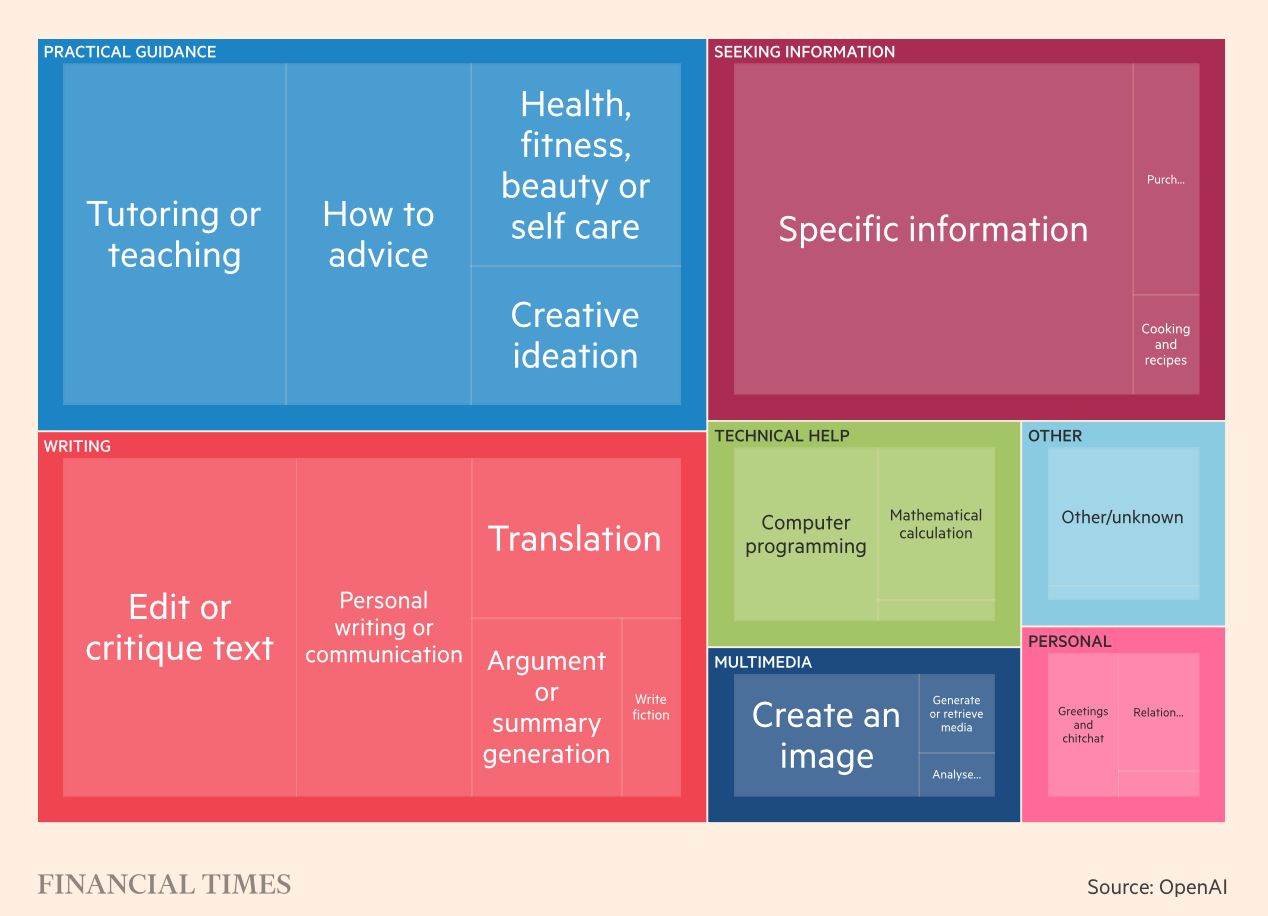
\includegraphics[width=10cm,totalheight=5cm]{figures/chatgpt}
\par\end{center}
\vspace{-3mm}
\begin{takeawaybox}\footnotesize
Consumer usage is dominated by \emph{generative} tasks --- writing, coding, tutoring, and open-ended Q\&A. But \emph{who} uses it, and for \emph{which} tasks, varies enormously across the economy --- something we can now measure directly. $\rightarrow$
\end{takeawaybox}
\end{frame}

\begin{frame}{How AI Is \emph{Actually} Used Within an Occupation}
\begin{center}
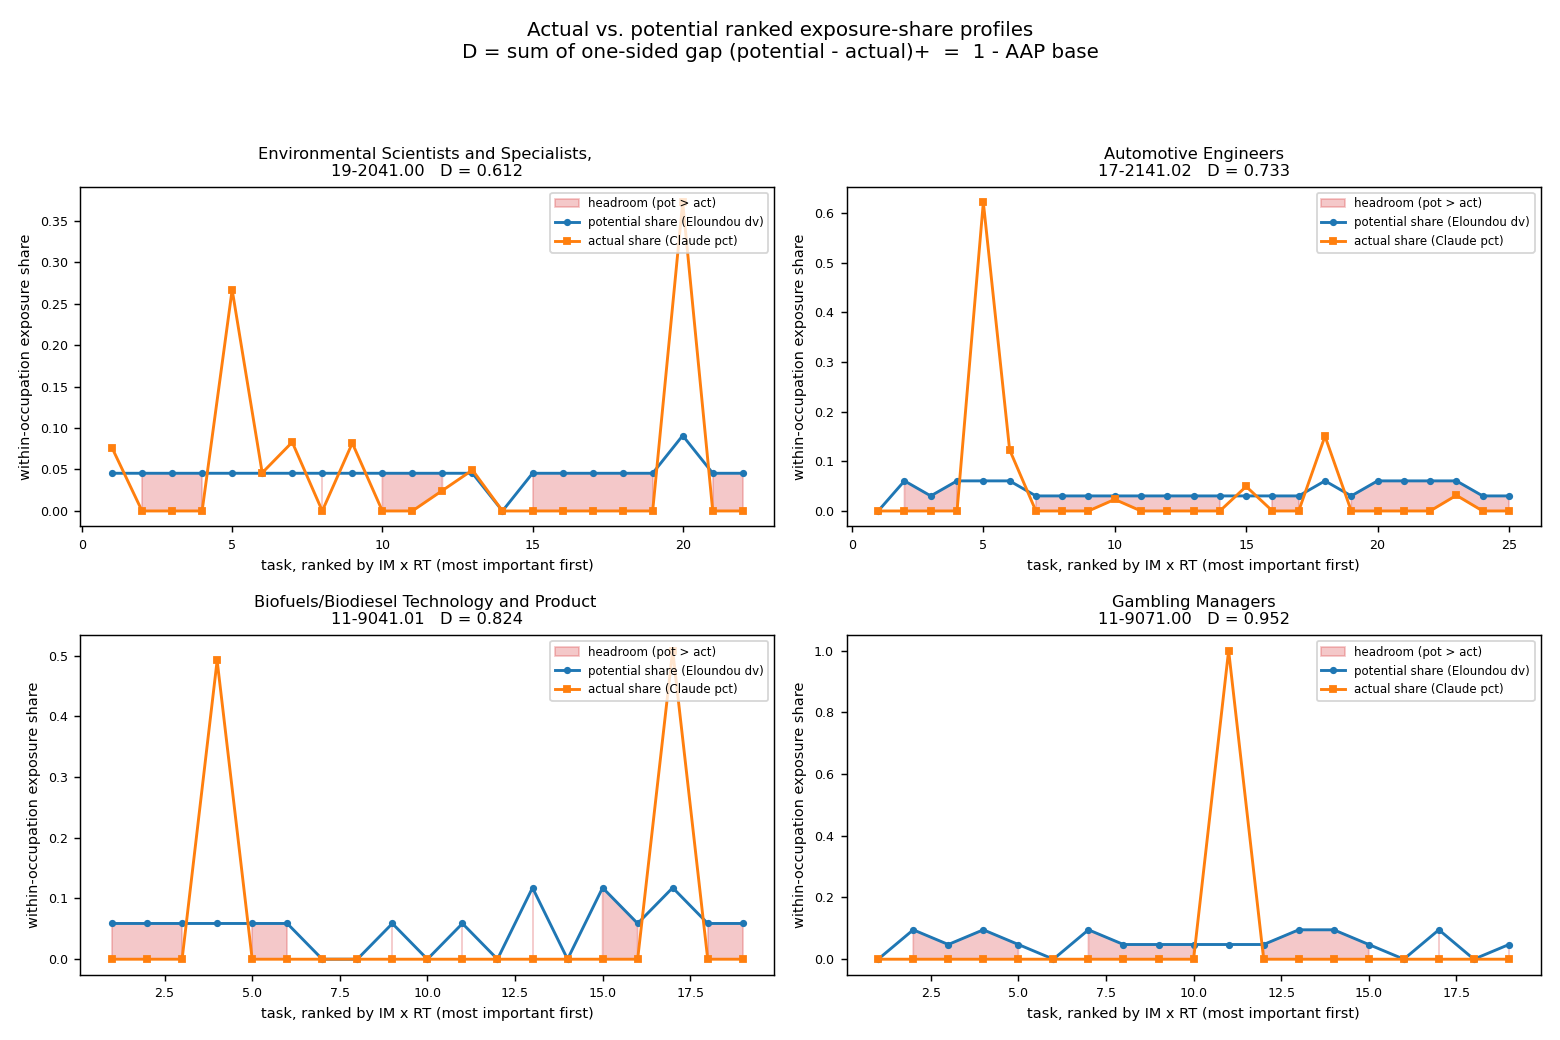
\includegraphics[width=12.2cm,totalheight=4.9cm,keepaspectratio]{figures/ranked_exposure_profiles}
\par\end{center}
\vspace{-1mm}
\begin{takeawaybox}\footnotesize
Each panel is one occupation; its tasks run along the $x$-axis, \emph{most important first}. \textbf{Orange $=$ where AI is actually used}; \textbf{blue $=$ where it \emph{could} be}. Actual use \emph{spikes on one or two tasks} and leaves the rest untouched --- and the pattern differs sharply by occupation.
\end{takeawaybox}
{\scriptsize\textit{Source: author's analysis --- Anthropic Economic Index (Claude usage) $\times$ O*NET importance $\times$ Eloundou et al.\ (2023).}}
\end{frame}

\begin{frame}{Zooming Out: AI-Usage Concentration Across 800+ Occupations}
\begin{center}
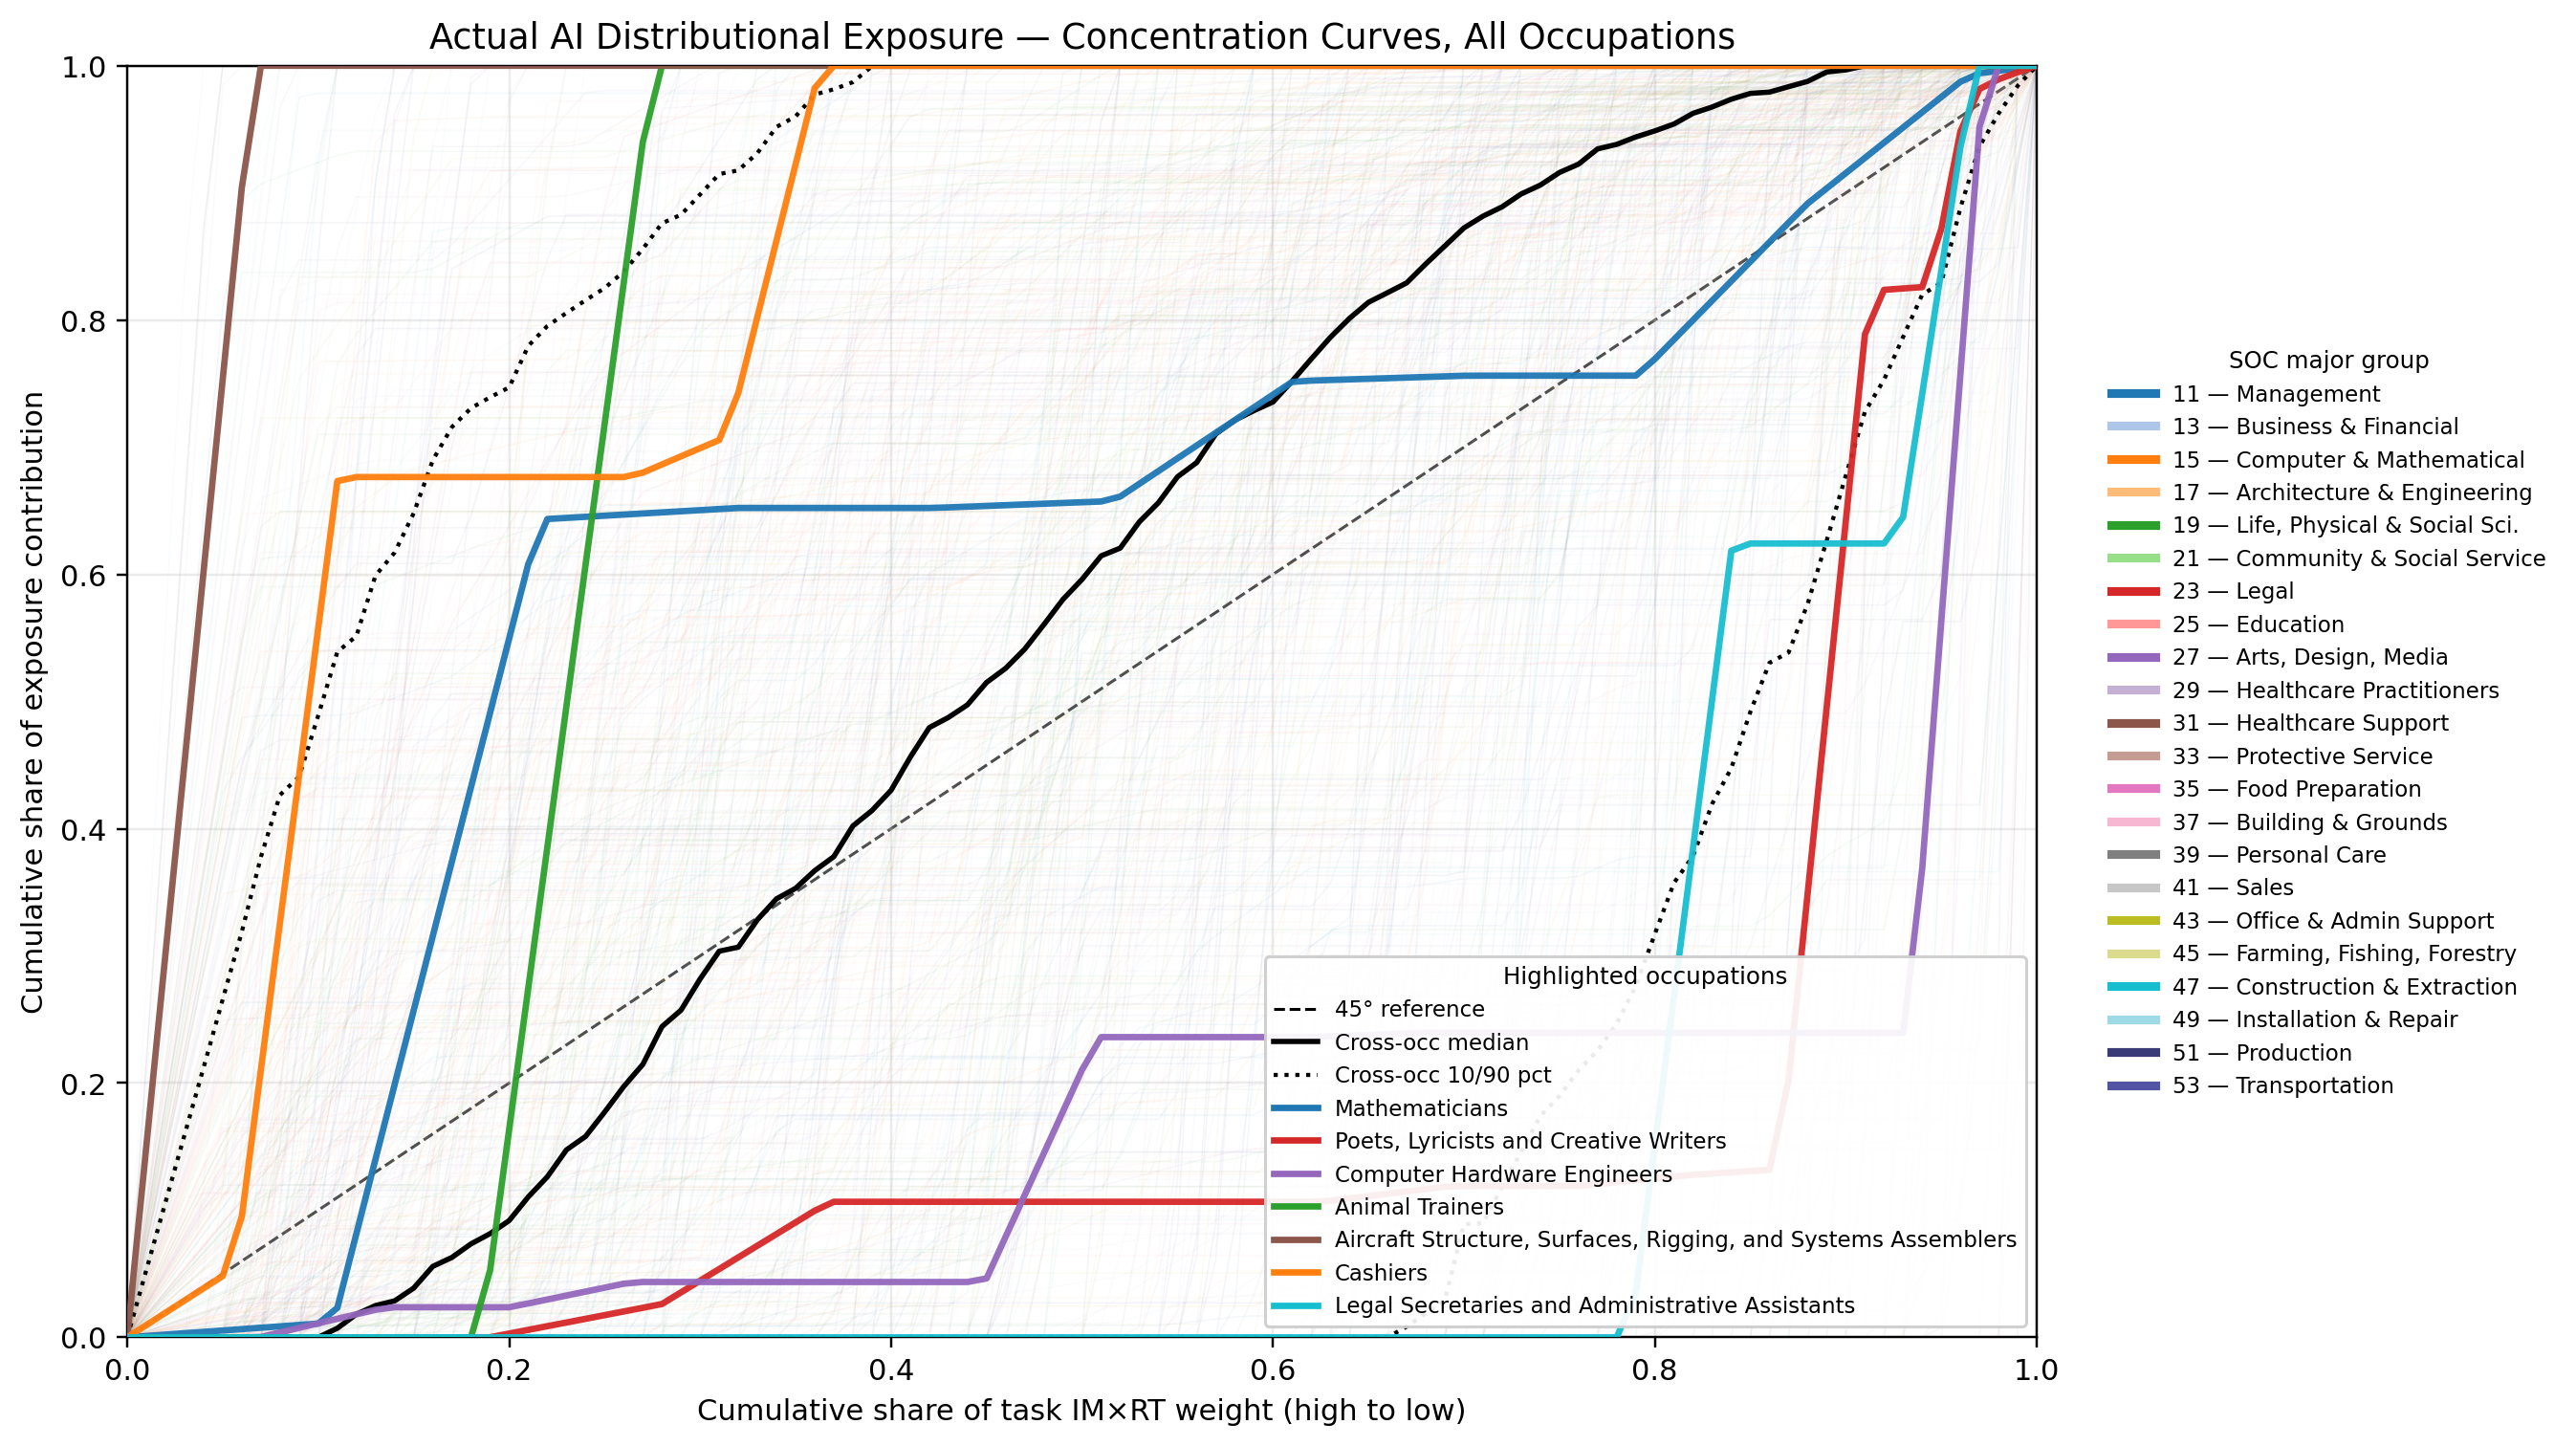
\includegraphics[width=12.2cm,totalheight=4.8cm,keepaspectratio]{figures/spaghetti_distributional_exposure_actual}
\par\end{center}
\vspace{-1mm}
\begin{takeawaybox}\footnotesize
Each faint line is one occupation's \emph{concentration curve} --- how fast AI usage accumulates as tasks are added most- to least-important. \emph{Above} the 45$^\circ$ line $=$ usage on \textbf{core} tasks (Cashiers, Mathematicians); \emph{below} $=$ on \textbf{peripheral} tasks. AI's footprint is highly uneven.
\end{takeawaybox}
{\scriptsize\textit{Source: author's analysis --- Anthropic Economic Index (Claude usage), 833 O*NET occupations.}}
\end{frame}

%=============================================================================
\section{Caution: Why Generative AI Still Fails}

\sectiondivider{Caution: Why Generative AI Still Fails}{Hallucination and deepfakes: it \emph{can}, but unreliably or harmfully}

\begin{frame}{Hallucination: Automating Plausibility, Not Truth}
\begin{itemize}
\item LLMs are trained to produce \emph{plausible} text, not \emph{true} statements: there is \textbf{no source of truth during training}. Fabrication is therefore \emph{inherent} --- not a bug a future patch removes.
\medskip
\item \textbf{Anchor (Mata v.\ Avianca, 2023):} a New York lawyer filed a ChatGPT-written brief that cited \textbf{entirely fabricated cases and invented judicial opinions}; asked whether they were real, the model insisted they were. The lawyer was sanctioned.
\medskip
\item \textbf{It is systematic, not a one-off:}
\begin{itemize}
    \item \textbf{CNET:} of 77 AI-written articles, \textbf{41 contained factual errors} --- despite a ``fact-checked'' label.
    \item \emph{Defamation by chatbot:} models have fabricated news stories accusing real people of crimes they never committed.
\end{itemize}
\end{itemize}
\begin{cautionbox}
\footnotesize
\textbf{Implication:} generative AI is \emph{unreliable for any high-stakes factual task} unless every claim is independently verified. \\[2pt] {\scriptsize Source for this section's cases: Narayanan \& Kapoor, \emph{AI Snake Oil} (2024).}
\end{cautionbox}
\end{frame}

\begin{frame}{Deepfakes \& Malicious Use: Capability Turned Against People}
\begin{itemize}
\item The same generative capability produces realistic \textbf{voice, image, and video} from seconds of source material.
\medskip
\item \textbf{Fraud (2019):} a UK energy firm's managing director wired $\approx$~EUR~220{,}000 to a fake supplier after a \textbf{voice-cloned call} impersonating his boss --- one of the first confirmed AI-enabled scams.
\medskip
\item \textbf{Non-consensual harm:} a single Telegram bot generated \textbf{100{,}000+ fabricated intimate images} of real women without their consent; the \emph{large majority} of harmful deepfakes target women this way (``image-based abuse'').
\medskip
\item \textbf{The ``liar's dividend'':} once \emph{anything} could be fake, real evidence can be waved away as fake too --- truth itself loses its anchor.
\end{itemize}
\begin{cautionbox}
\footnotesize
\textbf{Implication:} \emph{capability $\neq$ safety} --- a more capable generator is also a more capable weapon.
\end{cautionbox}
\end{frame}

\begin{frame}{Open Weights and the Safety Frontier: The DeepSeek Case}
\textbf{A genuine capability leap --- and a live case study in \emph{capability $\neq$ safety}.}
\smallskip
\begin{itemize}\footnotesize
    \item \textbf{The upside.} DeepSeek's open-weight models (V3, R1; 2025) matched frontier reasoning at a fraction of the cost --- exactly the ``open-source frontier'' that lowers the cost of academic experimentation.
    \item \textbf{The catch --- weak guardrails.} Independent red teams bypassed R1's safety filters with ease: Cisco reported a \emph{$\sim$100\% attack-success rate} on standard jailbreaks; others elicited malware, ransomware, and weapon-making instructions.
    \item \textbf{Open weights make safety \emph{optional}.} Anyone can download the weights and \emph{fine-tune the guardrails away}; safety that lives only inside the released model is not a real barrier (``illusory safety'').
    \item \textbf{Governance fallout.} Data stored under PRC jurisdiction, an exposed user-log database, and topic censorship led \emph{many governments} to ban it from official devices (Italy, Australia, South Korea, Taiwan, U.S.\ federal/state agencies).
\end{itemize}
\begin{cautionbox}\footnotesize
\textbf{For researchers:} open models are invaluable for reproducibility and cost --- but \emph{openness shifts the safety burden onto you}, the deployer. Capability, cost, and safety are \emph{separate} axes. \emph{(Status as of 2026; red-team findings from Cisco, KELA, Palo Alto Unit~42.)}
\end{cautionbox}
\end{frame}

\begin{frame}{The Practitioner's Discipline: What Task? What Data? What Claim?}
\begin{itemize}
\item \textbf{Reliability $\neq$ capability.} The two failure modes differ in kind:
\begin{itemize}
    \item \emph{Predictive failure} (T2.1): the model \textbf{can't} --- the future isn't in the data (COMPAS, Fragile Families).
    \item \emph{Generative failure} (this deck): the model \textbf{can, but unreliably or harmfully} (hallucination, deepfakes).
\end{itemize}
\medskip
\item \textbf{The habit that guards against both} --- before trusting any AI output, ask:
\begin{enumerate}
    \item \textbf{What task} is this, really? (a prediction? a generation? a decision?)
    \item \textbf{What data} did it learn from, and does my setting match?
    \item \textbf{What claim} am I making on its output, and how would I verify it?
\end{enumerate}
\end{itemize}
\begin{takeawaybox}
\footnotesize
AI is powerful \emph{but bounded}. We return to this discipline in \textbf{Lec.\ 7 T3b} (LLM limitations) and turn it into a publication-grade \textbf{audit checklist in Lec.\ 9 T5}.
\end{takeawaybox}
\end{frame}

\begin{frame}{The Same Discipline, for Economists}
\textbf{The three questions, sharpened for research use:}
\smallskip
\begin{enumerate}\footnotesize
    \item \textbf{What task?} Is the AI output a \emph{measurement} (a new variable), a \emph{prediction}, or a \emph{decision rule}? Each enters a paper differently --- and a measured variable is usually the most defensible.
    \medskip
    \item \textbf{What data?} Does the training distribution match \emph{your} sample and period? Watch for \emph{look-ahead / leakage} (a text model that already ``knows'' the outcome) and \emph{regime shifts} --- the Lucas-critique problem from T2.1.
    \medskip
    \item \textbf{What claim?} If an AI-generated variable sits on the \emph{right-hand side}, it carries \emph{measurement error} --- attenuation and generated-regressor problems. If it is the \emph{outcome}, validate it against ground truth on a held-out, human-coded sample.
\end{enumerate}
\begin{takeawaybox}\footnotesize
\textbf{Rule of thumb:} treat an AI output as an \emph{estimated input}, never as ground truth --- report the model, version, and prompt for \emph{reproducibility}, and robustness-check the AI step as you would any first-stage estimate. (Toolkit: Lec.\ 7--9.)
\end{takeawaybox}
\end{frame}

%=============================================================================
\begin{frame}{Lecture 2, Complete: One Map, Two Acts}
\textbf{You now hold the taxonomy: the predictive stack and the generative stack, each with its powers and its documented failure modes.}

\LecTwoMap{0}

\vspace{0.05cm}
\footnotesize\textit{The two acts now split into the course's two arcs: the predictive/RL stack drives Lec.\ 3--6 (dynamics); the generative stack drives Lec.\ 7--9 (language \& agents). Ask always: what task, what data, what claim.}
\end{frame}

\begin{frame}{Preview: What Lec.\ 3 Delivers}
\begin{itemize}
\item \textbf{Lec.\ 3 T1 --- Why ML for macro:} unstructured data (text, satellite, panels), curse of dimensionality, pattern recognition as motivation.

\medskip
\item \textbf{Lec.\ 3 T2 --- Neural networks:} architecture, activations (ReLU, sigmoid, tanh), universal approximation (Cybenko 1989, Hornik 1991).

\medskip
\item \textbf{Lec.\ 3 T3 --- Training:} forward/back propagation, gradient descent + AdamW, mini-batches, regularization (dropout, weight decay).

\medskip
\item \textbf{Lec.\ 3 T4 --- Specialized architectures:} ICNN, monotone NN, PICNN with macro shape restrictions.
\end{itemize}

\bigskip
\begin{center}
\footnotesize\textit{Lec.\ 3 is the toolkit; Lec.\ 4 turns it on the optimal-growth Bellman equation.}
\end{center}
\end{frame}

\begin{frame}{Summary}
\begin{enumerate}
\item \textbf{One stack, layered:} AI evolved from rule-based systems through ML and deep learning to today's generative and agentic era.

\medskip
\item \textbf{Three pillars of ML:} supervised (prediction), unsupervised (structure), reinforcement (sequential decisions) --- with deep learning as the shared engine.

\medskip
\item \textbf{Predictive AI fails} when the future is not in the data: COMPAS, Fragile Families --- proxies, gaming, and drift; the Lucas critique in ML clothing.

\medskip
\item \textbf{The generative stack:} NLP $\to$ LLMs $\to$ agents --- systems that \emph{generate} and \emph{act}, already woven into everyday and research use.

\medskip
\item \textbf{Generative AI fails differently:} it \emph{can}, but unreliably or harmfully --- hallucination, deepfakes; so always ask \emph{what task, what data, what claim}.

\medskip
\item \textbf{Next:} Lec.\ 3 goes hands-on with the dynamic-macro toolkit --- why ML for economists, neural networks, training, and specialized architectures.
\end{enumerate}
\end{frame}

\end{document}
